\section{Balance Workload}
Whenever a staff is removed from a department or has marked a problem as solved, 
it becomes necessary to balance the workload of each staff member in the department, since we do not want the staff members to be overloaded with problems. 

To balance the workload, each staffs workload must be calculated. 
The workload of a staff is defined by the amount of time estimated that each problem on his workload takes to be solved. 
The workload is calculated by the \me{GetWorkload} method.

The time a problem takes to be solved is estimated by the average time consumption of the tags connected to the problem. 
This is calculated by the \me{CalculateTimeConsumption} method.

The \me{BalanceWorkload} method works by finding the staff in the department with the minimum workload and the staff with the maximum workload. Then it moves the highest priority problems from the maximum staff to the minimum. 
It keeps reassigning problems until the minimum staff has a higher or equal workload than the maximum staff. If it is higher the problem is reassigned back. 

The original idea was that this would ensure that bad last reassignments would be omitted by switching them backwards. However, later we discovered that this approach is not sufficient to prevent bad last reassignments. An example is illustrated in figure \ref{fig:balanceWorkload_strangecase}. The dark grey colored box is representing a high priority problem which in the first scenario, the workload is most balanced if it is moved back after the final iteration of the loop, whereas the workload is most balanced if it is not moved back in on the scenario to the right, marked ``Move back Bad idea''. Although that this seems like a trivial bug to fix afterwards, we chose not to fix it, as it would make.
%%%%%%%%%%%%%%%%
----- ret efter at rasmus har omsrkevet funktionen
%%%%%%%%%%%%%%%%

All this is iterated once per staff minus one in the department. 
E.g. if there are two staffs it is ran once, if there is three it yields two etc. 
The pseudo code is displayed in code snippet \ref{lst:balanceWorkload}.

The primary concern of the algorithm is to distribute the problems so each staff has as balanced workload as possible.

 
%This balance is based on the time of all the individual staff members problems are approximated to take.
%This balance is based on the time approximated that all problems on his workload consumes. 
%							den tid alle de individuelle staff medlemmers problemer er approximeret til at tage, tilsammen.
%Balancen er baseret p\aa{} den tid alle staff problemer er approximeret til at tage tilsammen. 


We also wanted the algorithm to take the individual priority of the problems into account. 
This algorithm makes sure that the high priority problems will be distributed. 
If the priority was unrelevant the algorithm would take the problem with lowest time consume, since this would give the most balanced workload. 
An example of the algorithm is shown on figure \ref{fig:balanceWorkloadDiagram}. 

%There is one weakness though and that is if a staff has a highly time consuming problem with low priority. Then he will be left with only that problem. Assuming it is as time consuming as all the other problems. 



\begin{figure}
	\centering
		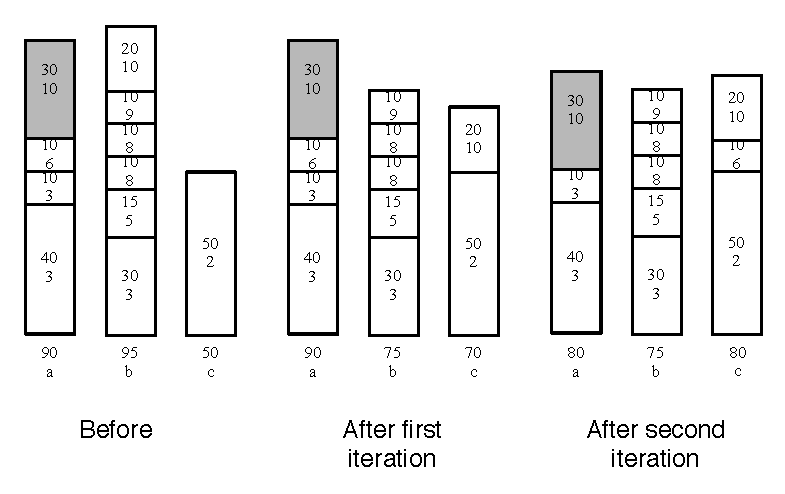
\includegraphics[scale=0.8]{input/implementation/key_points/balanceWorkloadDiagram.pdf}
	\morscaption{A diagram of the balance workload method. Each collumn represents a staffs workload. Each box is a problem. The upper number is the estimated time consumed of that problem. The lower is the priority. The problem colored dark grey is not reassignable.  There are tree staffs a, b, and c. The problems that will be moved is colored light grey. }
	\label{fig:balanceWorkloadDiagram}
\end{figure}

\begin{figure}
	\centering
		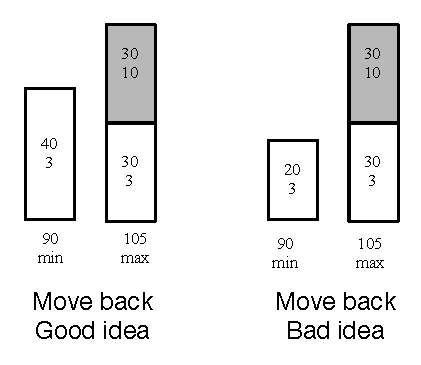
\includegraphics[scale=1.0]{input/implementation/key_points/balanceWorkload_strangecase.pdf}
	\morscaption{Diagram illustrating the result of the \me{BalanceWorkload} method, executed in two different scenarios, where the final ``moveback'' in the loop is good and bad idea.}
	\label{fig:balanceWorkload_strangecase}
\end{figure}


\begin{lstlisting}[style=sourceCode, caption=\myCaption{A code snippet of the balance workload method. The presented code is within a for loop running each for every staff minus one}, label=lst:balanceWorkload]
var max = Persons.FirstOrDefault(y => 	
		y.GetWorkload() == Persons.Max(x => 
		x.GetWorkload()));                  

var min = Persons.FirstOrDefault(y => 
		y.GetWorkload() == Persons.Min(x => 
		x.GetWorkload()));

// Sorts the list after priority
max.Worklist.ToList().Sort(Problem.GetComparer());             
while(true)
{
    var problemToBeMoved = max.Worklist.FirstOrDefault(y => 
		y.Reassignable == true && 
		y.HasBeen == false && 
		y.SolvedAtTime == null);
                   
    if (problemToBeMoved == null)     break; 
    problemToBeMoved.HasBeen = true;
    problemToBeMoved.AssignedTo = min;
    
    if (min.Workload > max.Workload)
    {
	    // Move problem back
    	problemToBeMoved.AssignedTo = max;
    	break;
    }
    else if (min.Workload == max.Workload)
    {
		break;
    }
} 
\end{lstlisting}




\subsection{eta}
\label{}


Get workload kalder ETA